\section*{Chuncked LOD}
  \label{sec:chunked-lod}

  
  la méthode \textit{CLOD} "Chuncked LOD" développé par Thatcher Ulrich~\cite{CLOD}, sur laquelle est basé la méthode \textit{CDLOD}.

\begin{figure}[!ht]
\centerline{
    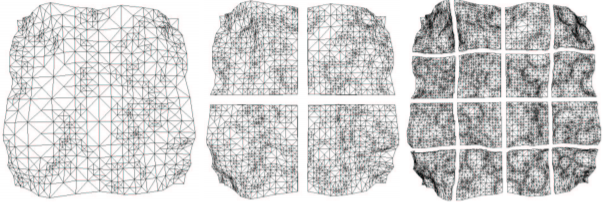
\includegraphics[width=11cm,height=3.5cm]{img/clod.png}}
    \caption[CLOD]{CLOD\protect\footnotemark}
    \label{fig:clod}
\end{figure}
\footnotetext{Extrait de \url{http://tulrich.com/geekstuff/sig-notes.pdf}, dernier accès Mars 2018}


  La méthode \emph{CLOD} utilise un \textit{quadtree} permettant de stocker les différents \emph{LOD}. Lors de l'exécution le \emph{quadtree} est généré et composé des niveaux de détails, les \emph{LOD} nécessaire sont calculés et ainsi utilisés depuis le \emph{quadtree}. 
  
  Pour appliquer une texture il suffit alors d'associer chaque "chunck" (n\oe{}ud) à une texture.
  Le rendue du terrain est alors fait en fonction de la distance par rapport à la caméra. Pour affiché un n\oe{}ud, le \emph{quadtree} est parcourue depuis la racine avec une tolérance maximum prédéfinie. Si le du n\oe{}ud parcourue est valide il est affiché et si il y a un trop grand écart alors on vérifie ses fils dans \emph{quadtree}, et ainsi de suite.
 
  Lorsqu'un n\oe{}ud est sur le point d'être réduit à ses fils ou inversement, il va alors se produire un effet "flash"/une apparition brusque de la grille. La méthode résout se problème en ajoutant un petit \emph{morphing} (une transition fluide). Pour se faire la méthode utilisé consiste à ajouter un point et de le décaler pour que cela corresponde niveau de détail souhaité(plus grand ou plus petit)
 
 
 \begin{figure}[!ht]
 \centerline{
    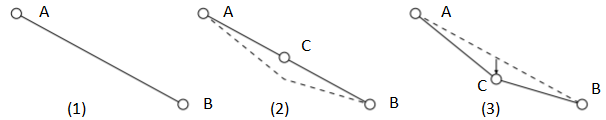
\includegraphics[width=8cm,height=2cm]{img/morph-pop.png}}
    \caption[morph]{ Illustration \protect\footnotemark}
    \label{fig:morph-pop}
\end{figure}
\footnotetext{Extrait de \url{http://tulrich.com/geekstuff/sig-notes.pdf}, dernier accès Mars 2018}

\newpage
  Dans l'exemple de la figure \ref{fig:morph-pop} la ligne (1) est composé de deux sommets (A et B),on cherche ensuite à augmenter le niveau de détail de cette ligne en y ajoutant un sommet. On va donc placer un troisième sommet (C) au milieu de la ligne composant donc une ligne plus détaillé (2). Le troisième sommet ainsi placé va ensuite être déplacé progressivement pour atteindre son propre emplacement, et représenter le "bon détail" (3).\\

 Un nouveau problème va donc par la suite apparaître. Comme montré et expliqué au début du chapite \ref{chap:cdlod}, la différence entre deux niveaux de détails voisins va faire apparaître des discontinuité. Ulritch.T pour se faire va alors en quelque sorte "remplir" ces trous en créant un "rideau" composé de la même texture dont il va se servir pour combler le vide entre les n\oe{}uds.
 Le premier problème de cette méthode est que pour s'assurer que le "rideau" couvre la totalité de la zone vide, ce dernier doit partir de la plus grande hauteur de la zone et descendre à la vertical en dessous de la totalité du niveau de détail. C'est à dire peut-être(et même dans la plus part du temps) au dessous du niveau actuel. Cela va donc crée une zone affiché mais non visible.

 \begin{figure}[!ht]
    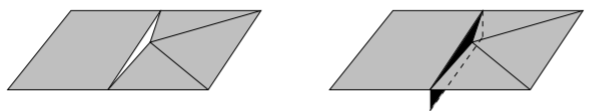
\includegraphics[width=12cm]{img/skirt.png}
    \caption[morph]{ Résolution du problème de discontinuité \protect\footnotemark}
    \label{fig:skirt}
\end{figure}
\footnotetext{Extrait de \url{http://tulrich.com/geekstuff/sig-notes.pdf}, dernier accès Mars 2018}

Dans l'exemple de la figure \ref{fig:skirt}, sur la figure de gauche, une discontinuité est apparue car la zone de gauche est à un niveau plus haut que le point formé par la zone de droite, qui après avoir glisser(comme vue dans l'exemple de la figure \ref{fig:morph-pop}) va se situer plus bas est crée un vide.
Le rideau va ainsi se créer (visible sur la figure de droite). On peut ainsi bien observer que le rideau va au delà de la discontinuité.

Le deuxième problème de cette méthode, est que la texture appliqué à se rideau est la même que l'arête où se produit la discontinuité. Il n'y aura donc en effet pas de zone vide, mais la texture en elle même ne serra pas propre au triangle.